\documentclass[aspectratio=169, table]{beamer}

\usepackage{colortbl}
\usepackage{xcolor}
\usepackage{listings}
\usepackage{tikz}
\usepackage{pgfplots}
\usepgfplotslibrary{polar}
\usetikzlibrary{arrows.meta, positioning, calc, backgrounds}

\usetheme{Pradita}



\lstdefinelanguage{bash} {
	keywords={},
	basicstyle=\ttfamily\scriptsize,
	keywordstyle=\color{blue}\bfseries,
	ndkeywords={iex},
	ndkeywordstyle=\color{purple}\bfseries,
	sensitive=true,
	commentstyle=\color{gray},
	stringstyle=\color{red},
	numbers=left,
	numberstyle=\tiny\color{gray},
	breaklines=true,
	frame=lines,
	backgroundcolor=\color{lightgray!10},
	tabsize=2,
	comment=[l]{\#},
	morecomment=[s]{/*}{*/},
	commentstyle=\color{gray}\ttfamily,
	stringstyle=\color{purple}\ttfamily,
	showstringspaces=false,
	captionpos=b
}

% Define Python language style for listings
\lstdefinestyle{PythonStyle}{
    language=Python,
    basicstyle=\ttfamily\footnotesize,
    keywordstyle=\color{blue}\bfseries,
    commentstyle=\color{gray}\itshape,
    stringstyle=\color{red},
    showstringspaces=false,
    breaklines=true,
    frame=lines,
    numbers=left,
    numberstyle=\tiny\color{gray},
    backgroundcolor=\color{lightgray!10},
    tabsize=4,
    captionpos=b
}


\subtitle{IT30213 - Advanced Software Engineering \& DevOps}
\title{\Huge Continuous Integration \\
	and Deployment\vspace{8pt}}
%\date[Serial]{Penggunaan Large Language Model untuk Pengajaran}
\author{\textbf{Alfa Yohannis}}
\begin{document}
	
	\frame{\titlepage}
	

	\begin{frame}[fragile]
		\frametitle{Contents}
		\vspace{20pt}
		\begin{columns}[t]
			\column{0.5\textwidth}
			\tableofcontents[sections={1-5}]
			
			\column{0.5\textwidth}
			\tableofcontents[sections={6-20}]
		\end{columns}
	\end{frame}
	
	\begin{frame}{\hfill}
		\centering
		\Huge{\textbf{What can we do to secure our software systems?}}
	\end{frame}
	
\section{Pendahuluan}

	\begin{frame}{\hfill}
		\centering
		\Huge{\textbf{Pendahuluan}}
	\end{frame}

\begin{frame}{Pendahuluan}
	\vspace{6pt}
	\begin{itemize}
		\item Pengembangan perangkat lunak modern bersifat \textbf{kontinu dan kolaboratif}, khususnya pada sistem terdistribusi dengan banyak layanan.
		\item Setiap perubahan kode dapat memengaruhi lebih dari satu komponen, sehingga integrasi manual meningkatkan risiko kesalahan.
		\item CI/CD hadir untuk menjaga kualitas sistem tanpa mengorbankan kecepatan pengembangan.
		\item Melalui pipeline otomatis, integrasi, pengujian, dan penyebaran dijalankan secara konsisten dan terverifikasi.
		\item Bab ini menerapkan konsep CI/CD pada studi kasus sistem \textit{text-to-speech} berbasis layanan terdistribusi.
	\end{itemize}
\end{frame}


\section{Apa yang Dimaksud dengan CI/CD?}

	\begin{frame}{\hfill}
		\centering
		\Huge{\textbf{Apa yang Dimaksud dengan CI/CD?}}
	\end{frame}

\begin{frame}{Apa yang Dimaksud dengan CI/CD?}
	\vspace{6pt}
	\begin{itemize}
		\item CI/CD adalah pendekatan untuk \textbf{mengotomatisasi} integrasi kode, pengujian, dan penyebaran aplikasi.
		\item \textit{Continuous Integration} (CI) mengintegrasikan setiap perubahan kode secara rutin ke repository pusat dan memicu build serta pengujian otomatis.
		\item CI membantu mendeteksi kesalahan lebih awal sebelum masalah berkembang lebih kompleks.
		\item \textit{Continuous Delivery} (CD) memastikan hasil integrasi selalu berada dalam kondisi siap untuk dideploy.
		\item \textit{Continuous Deployment} melanjutkan CD dengan mendeploy setiap perubahan yang lolos CI secara otomatis.
		\item Dalam praktik modern, CI/CD juga mencakup build container dan pengujian integrasi.
	\end{itemize}
\end{frame}



\section{Workflow CI/CD}

	\begin{frame}{\hfill}
		\centering
		\Huge{\textbf{Workflow CI/CD}}
	\end{frame}

\begin{frame}{Workflow CI/CD}
	\vspace{6pt}
	\begin{itemize}
		\item Workflow CI/CD adalah urutan langkah terotomatisasi yang dijalankan setiap kali terjadi perubahan kode.
		\item Workflow didefinisikan secara deklaratif (misalnya YAML) dan dieksekusi oleh sistem otomasi seperti GitHub Actions.
		\item Proses dimulai dari \textit{checkout} kode dan penyiapan lingkungan eksekusi yang konsisten.
		\item Pengujian unit dan integrasi dijalankan untuk memverifikasi bahwa perubahan tidak merusak sistem.
		\item Kegagalan pada satu tahap akan menghentikan workflow dan memberi umpan balik langsung.
		\item Deployment hanya dijalankan untuk artefak yang telah lolos seluruh tahapan CI.
	\end{itemize}
\end{frame}


\begin{frame}{Workflow CI/CD pada Studi Kasus}
	\vspace{6pt}
	\begin{columns}[T]
		\column{0.55\textwidth}
		\vspace{20pt}
		\begin{itemize}
			\item Perubahan kode melalui \textit{commit}, \textit{push}, atau \textit{pull request} memicu workflow CI.
			\item Workflow CI menjalankan pengujian unit dan integrasi secara otomatis pada runner GitHub-hosted.
			\item Hanya perubahan yang lolos CI (\texttt{success}) yang dapat melanjutkan ke tahap deployment.
			\item Deployment dijalankan melalui workflow terpisah pada \textit{self-hosted runner}.
			\item Dengan mekanisme ini, sistem yang berjalan selalu berasal dari kode yang telah diverifikasi.
		\end{itemize}

		\column{0.45\textwidth}
		\vspace{-23pt}
		\centering
		\scalebox{0.62}{%
		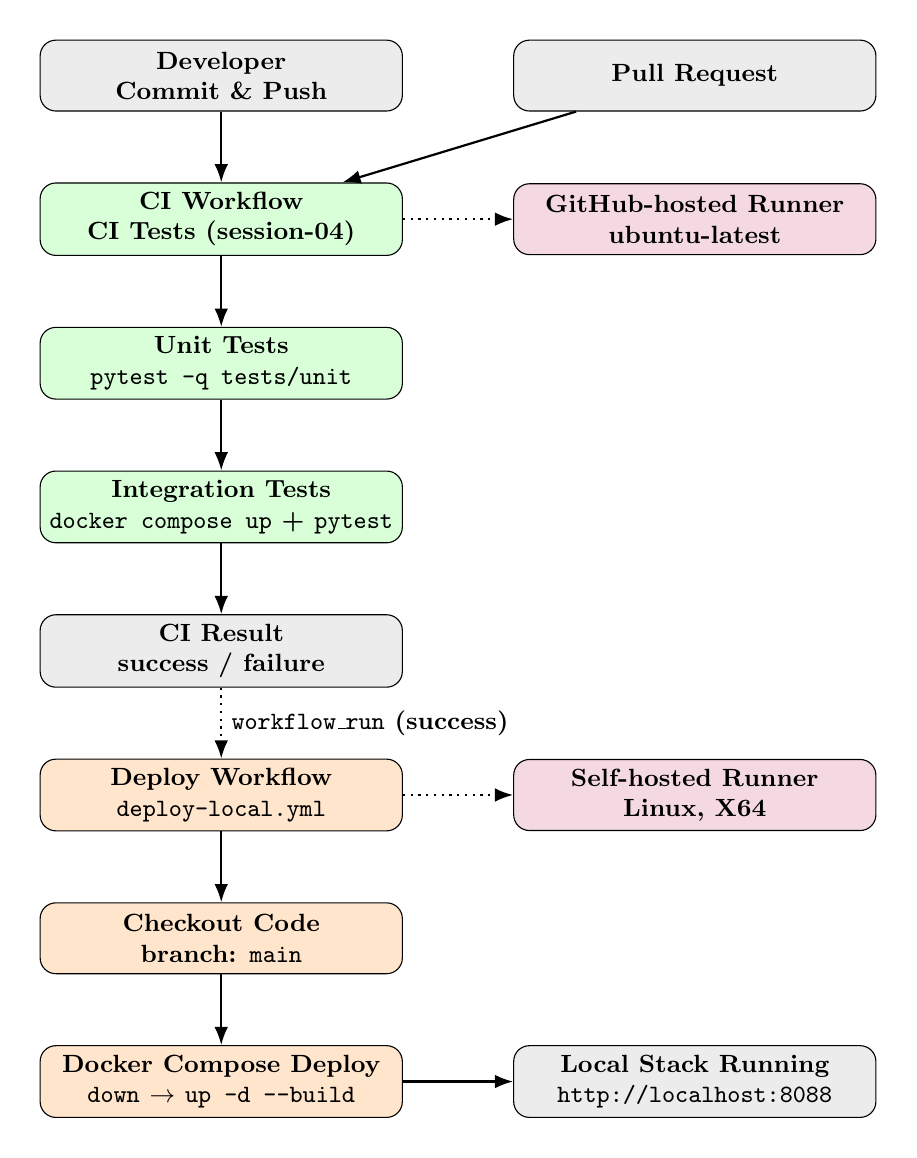
\begin{tikzpicture}[
		  background rectangle/.style={fill=white},
		  show background rectangle,
		  font=\small\bfseries,
		  node distance=9mm,
		  box/.style={
		    draw,
		    rounded corners=2mm,
		    align=center,
		    minimum width=46mm,
		    minimum height=9mm,
		    fill=blue!10
		  },
		  eventbox/.style={box,fill=gray!15},
		  cibox/.style={box,fill=green!15},
		  deploybox/.style={box,fill=orange!20},
		  runnerbox/.style={box,fill=purple!15},
		  arrow/.style={-Latex,thick},
		  dottedarrow/.style={-Latex,thick,dotted}
		]

		% --- top events ---
		\node[eventbox] (dev) {Developer\\Commit \& Push};
		\node[eventbox, right=14mm of dev] (pr) {Pull Request};

		% --- CI pipeline ---
		\node[cibox, below=of dev] (ci) {CI Workflow\\CI Tests (session-04)};
		\node[runnerbox, right=14mm of ci] (ghrunner) {GitHub-hosted Runner\\ubuntu-latest};

		\node[cibox, below=of ci] (unit) {Unit Tests\\\texttt{pytest -q tests/unit}};
		\node[cibox, below=of unit] (integ) {Integration Tests\\\texttt{docker compose up} + \texttt{pytest}};
		\node[eventbox, below=of integ] (result) {CI Result\\success / failure};

		% --- deploy pipeline ---
		\node[deploybox, below=of result] (deploywf) {Deploy Workflow\\\texttt{deploy-local.yml}};
		\node[runnerbox, right=14mm of deploywf] (self) {Self-hosted Runner\\Linux, X64};

		\node[deploybox, below=of deploywf] (checkout) {Checkout Code\\branch: \texttt{main}};
		\node[deploybox, below=of checkout] (deploy) {Docker Compose Deploy\\\texttt{down} $\rightarrow$ \texttt{up -d --build}};
		\node[eventbox, right=14mm of deploy] (running) {Local Stack Running\\\texttt{http://localhost:8088}};

		% --- arrows ---
		\draw[arrow] (dev) -- (ci);
		\draw[arrow] (pr) -- (ci);

		\draw[dottedarrow] (ci) -- (ghrunner);
		\draw[arrow] (ci) -- (unit);
		\draw[arrow] (unit) -- (integ);
		\draw[arrow] (integ) -- (result);

		\draw[dottedarrow] (result) -- node[right]{\texttt{workflow\_run} (success)} (deploywf);
		\draw[dottedarrow] (deploywf) -- (self);

		\draw[arrow] (deploywf) -- (checkout);
		\draw[arrow] (checkout) -- (deploy);
		\draw[arrow] (deploy) -- (running);

		\end{tikzpicture}%
		}
	\end{columns}
\end{frame}

\section{Contoh Studi Kasus}

	\begin{frame}{\hfill}
		\centering
		\Huge{\textbf{Contoh Studi Kasus}}
	\end{frame}


\begin{frame}{Arsitektur Sistem TTS (Studi Kasus)}
	\vspace{20pt}
	\centering
	\scalebox{0.8}{
	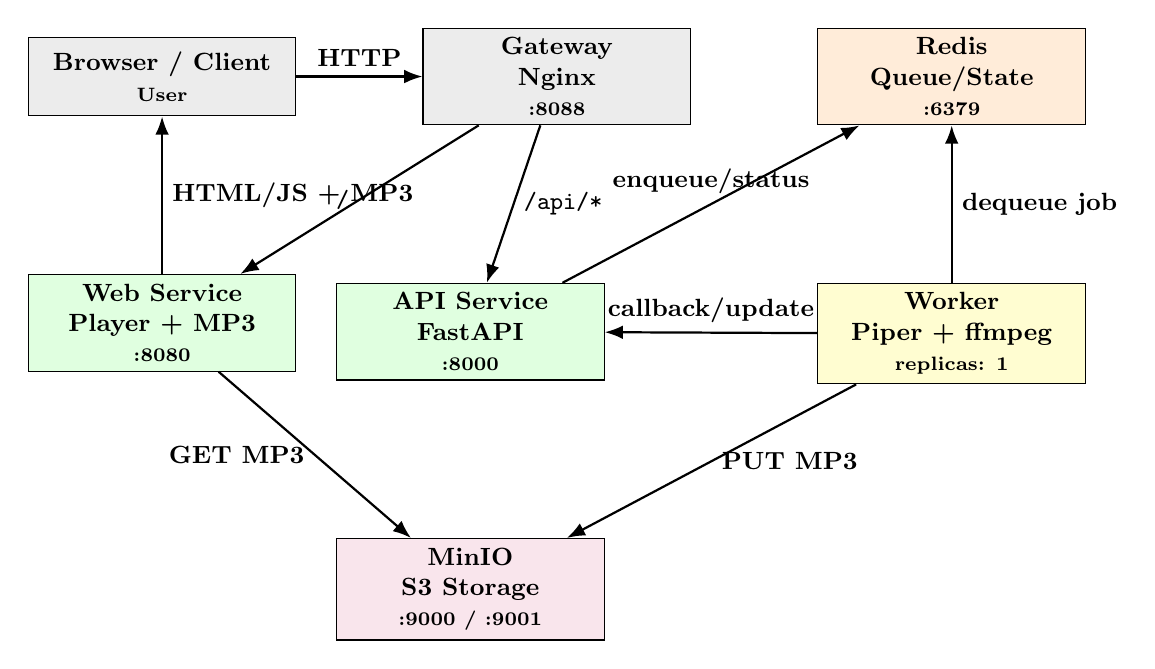
\begin{tikzpicture}[
	  font=\small\bfseries,
	  node distance=20mm and 16mm,
	  box/.style={
	    draw,
	    align=center,
	    minimum width=34mm,
	    minimum height=10mm,
	    fill=blue!10
	  },
	  storebox/.style={box,fill=purple!10},
	  brokerbox/.style={box,fill=orange!15},
	  apiwebbox/.style={box,fill=green!12},
	  gatewaybox/.style={box,fill=gray!15},
	  workerbox/.style={box,fill=yellow!18},
	  annot/.style={font=\scriptsize\itshape, text=black!70},
	  arrow/.style={-Latex,thick}
	]

	% --- Row 1 (top) ---
	\node[gatewaybox] (client) {Browser / Client\\{\scriptsize User}};
	\node[gatewaybox, right=of client] (gateway) {Gateway\\Nginx\\{\scriptsize :8088}};
	\node[brokerbox, right=of gateway] (redis) {Redis\\Queue/State\\{\scriptsize :6379}};

	% --- Row 2 (middle) ---
	\node[apiwebbox, below=of client] (web) {Web Service\\Player + MP3\\{\scriptsize :8080}};
	\node[apiwebbox, below=of gateway, xshift=-11mm] (api) {API Service\\FastAPI\\{\scriptsize :8000}};
	\node[workerbox, below=of redis] (worker) {Worker\\Piper + ffmpeg\\{\scriptsize replicas: 1}};

	% --- Row 3 (bottom) ---
	\node[storebox, below=of api] (minio) {MinIO\\S3 Storage\\{\scriptsize :9000 / :9001}};

	% --- Flows ---
	\draw[arrow] (client) -- node[above]{HTTP} (gateway);
	\draw[arrow] (gateway) -- node[left]{\texttt{/}} (web);
	\draw[arrow] (gateway) -- node[right]{\texttt{/api/*}} (api);
	\draw[arrow] (api) -- node[above]{enqueue/status} (redis);
	\draw[arrow] (worker) -- node[right]{dequeue job} (redis);
	\draw[arrow] (worker) -- node[above]{callback/update} (api);
	\draw[arrow] (worker) -- node[right]{PUT MP3} (minio);
	\draw[arrow] (web) -- node[left]{GET MP3} (minio);
	\draw[arrow] (web) -- node[right]{HTML/JS + MP3} (client);

	\end{tikzpicture}
	}
\end{frame}

\begin{frame}{Penjelasan Studi Kasus TTS (docker-compose)}
	\vspace{6pt}
	\begin{itemize}
		\item Sistem TTS dijalankan lokal dengan \texttt{docker-compose}; diagram menjelaskan relasi layanan dan alur data end-to-end.
		\item Klien mengakses \textit{gateway} Nginx (\texttt{:8088}) yang merutekan \texttt{/} ke \textit{web} dan \texttt{/api/*} ke \textit{api}.
		\item \textit{API} (FastAPI) memvalidasi permintaan dan mengantrikan job ke Redis (\texttt{jobs:queue:dev}) agar pemrosesan asinkron.
		\item \textit{Worker} mengambil job, menjalankan Piper + \texttt{ffmpeg}, lalu menyimpan MP3 ke MinIO (S3); worker bersifat stateless.
		\item \textit{Web} menyajikan UI dan mengambil MP3 dari MinIO untuk diputar; dependensi layanan diatur eksplisit di \texttt{docker-compose.yml}.
	\end{itemize}
\end{frame}

\begin{frame}[fragile]{Menjalankan Sistem dengan Docker Compose}
	\vspace{4pt}
	\begin{columns}[T]
		\column{0.6\textwidth}
		\begin{lstlisting}[language=bash]
# stop old containers (avoid port/state conflicts)
sudo docker compose down

# rebuild images
sudo docker compose build

# start all services
sudo docker compose up
		\end{lstlisting}

		\column{0.4\textwidth}
		\begin{itemize}
			\item Pastikan tidak ada container lama yang berjalan.
			\item Seluruh service dibangun ulang dari Dockerfile.
			\item API, web, worker, Redis, MinIO, dan gateway berjalan bersamaan.
			\item Log ditampilkan langsung di terminal.
		\end{itemize}
	\end{columns}
\end{frame}

\begin{frame}[fragile]{Mengakses API dan Web}
	\vspace{4pt}
	\begin{columns}[T]
		\column{0.6\textwidth}
		\begin{lstlisting}[language=bash]
# submit a text
curl -X POST http://localhost:8088/api/jobs \
  -H "Content-Type: application/json" \
  -d '{"text":"Hello world this is a test"}'

# get job status/result
curl http://localhost:8088/api/jobs/<job-id>

# access MP3 result
curl -I http://localhost:8088/mp3/<job-id>.mp3

# open web UI
http://localhost:8088/
		\end{lstlisting}

		\column{0.4\textwidth}
		\begin{itemize}
			\item Gateway Nginx menjadi satu-satunya entry point (\texttt{:8088}).
			\item API bersifat asinkron: request menghasilkan \textit{job ID}.
			\item MP3 dapat diakses via API maupun browser.
			\item Sistem dapat digunakan API-centric atau web-centric.
		\end{itemize}
	\end{columns}
\end{frame}

\section{Demo}

	\begin{frame}{\hfill}
		\centering
		\Huge{\textbf{Demo}}
	\end{frame}


\begin{frame}[fragile]{Demo (1/6): Akun dan Git}
	\vspace{4pt}
	\begin{itemize}
		\item GitHub digunakan sebagai pusat kode dan CI/CD.
		\item Git wajib tersedia dan terkonfigurasi secara global.
	\end{itemize}

	\vspace{4pt}
	\begin{lstlisting}[language=bash]
sudo apt update
sudo apt install -y git
git config --global user.name "Nama Anda"
git config --global user.email "email@contoh.com"
git --version
	\end{lstlisting}
\end{frame}

\begin{frame}[fragile]{Demo (2/6): Repository dan GitHub CLI}
	\vspace{4pt}
	\begin{itemize}
		\item Repository modul digunakan sebagai basis praktikum.
		\item GitHub CLI mempermudah autentikasi dan observasi workflow.
	\end{itemize}

	\vspace{4pt}
	\begin{lstlisting}[language=bash]
git clone https://github.com/alfa-yohannis/advanced-software-engineering.git
cd advanced-software-engineering

sudo apt install -y gh
gh auth login
gh auth status
	\end{lstlisting}
\end{frame}

\begin{frame}[fragile]{Demo (3/6): Docker dan Docker Compose}
	\vspace{4pt}
	\begin{itemize}
		\item Docker menjadi unit eksekusi utama sistem.
		\item Docker Compose menjalankan sistem multi-service.
	\end{itemize}

	\vspace{4pt}
	\begin{lstlisting}[language=bash]
sudo apt install -y docker.io docker-compose-plugin
sudo usermod -aG docker $USER
# logout & login kembali

docker version
docker compose version
	\end{lstlisting}
\end{frame}

\begin{frame}[fragile]{Demo (4/6): Self-hosted Runner}
	\vspace{4pt}
	\begin{itemize}
		\item Runner disiapkan untuk workflow deploy.
		\item Runner berjalan langsung di lingkungan target.
	\end{itemize}

	\vspace{4pt}
	\begin{lstlisting}[language=bash]
mkdir actions-runner && cd actions-runner

curl -O -L https://github.com/actions/runner/releases/download/v2.331.0/actions-runner-linux-x64-2.331.0.tar.gz
tar xzf actions-runner-linux-x64-2.331.0.tar.gz

./config.sh --url https://github.com/alfa-yohannis/advanced-software-engineering \
            --token <TOKEN>
./run.sh
	\end{lstlisting}
\end{frame}

\begin{frame}[fragile]{Demo (5/6): CI ke Deployment}
	\vspace{4pt}
	\begin{itemize}
		\item Commit dan push memicu workflow CI.
		\item CI sukses memicu deploy melalui \texttt{workflow\_run}.
	\end{itemize}

	\vspace{4pt}
	\begin{lstlisting}[language=bash]
git status
git add .
git commit -m "update config"
git push origin main

gh workflow list
gh run list --workflow "CI Tests (session-04)"
gh run list --workflow "CI Tests (session-04) --branch main --limit 1 --json databaseId --jq '.[0].databaseId'
gh run watch --exit-status
	\end{lstlisting}
\end{frame}

\begin{frame}[fragile]{Demo (6/6): Dari CI Sukses ke Deployment}
	\vspace{20pt}
	\begin{itemize}
		\item Workflow CI berakhir dengan status \texttt{success} jika lulus unit dan integration tests.
		\item Setelah CI selesai, GitHub memancarkan event \texttt{workflow\_run} dengan status \texttt{completed}.
		\item Event \texttt{workflow\_run} digunakan sebagai pemicu formal untuk workflow deploy.
		\item Workflow deploy hanya dijalankan jika hasil CI adalah \texttt{success}.
		\item Job deploy menargetkan \textbf{self-hosted runner} yang memiliki akses langsung ke lingkungan target.
		\item Runner \textbf{idealnya} melakukan \textit{checkout} branch \texttt{main} agar kode yang dideploy identik dengan kode yang diuji. \textbf{Untuk demo}, contoh ini langsung \textit{build }\& \textit{run} kode lokal.
	\end{itemize}
	\begin{lstlisting}[language=bash, basicstyle=\ttfamily\scriptsize]
- name: Run app locally (compose)
  run: |
    docker compose -f projects/session-04/docker-compose.yml down || true
    docker compose -f projects/session-04/docker-compose.yml up -d --build
    docker compose -f projects/session-04/docker-compose.yml ps
	\end{lstlisting}
\end{frame}


\section{Diskusi}

	\begin{frame}{\hfill}
		\centering
		\Huge{\textbf{Diskusi}}
	\end{frame}

\begin{frame}{Diskusi}
	\vspace{6pt}
	\begin{itemize}
		\item \textbf{Apa peran utama CI/CD dalam pengembangan perangkat lunak modern?}
		      Menghubungkan perubahan kode dengan proses verifikasi dan deployment secara otomatis dan konsisten.
		\item \textbf{Mengapa CI perlu menjalankan build, unit test, dan integration test?}
		      Untuk mendeteksi bug dan masalah integrasi sejak dini sebelum kode dirilis.
		\item \textbf{Di mana kegagalan paling sering muncul pada sistem terdistribusi?}
		      Pada batas antar layanan, bukan pada fungsi atau komponen tunggal.
		\item \textbf{Mengapa event \texttt{workflow\_run} penting dalam pipeline CI/CD?}
		      Karena memastikan deployment hanya dijalankan setelah CI berhasil.
		\item \textbf{Mengapa deployment dijalankan pada self-hosted runner?}
		      Agar proses deploy memiliki akses langsung ke lingkungan target dan Docker runtime.
	\end{itemize}
\end{frame}


\section{Ringkasan}

	\begin{frame}{\hfill}
		\centering
		\Huge{\textbf{Ringkasan}}
	\end{frame}

\begin{frame}{Ringkasan}
	\vspace{6pt}
	\begin{itemize}
		\item CI/CD menghubungkan perubahan kode dengan proses verifikasi dan deployment secara otomatis dan konsisten.
		\item CI menjalankan build, unit test, dan integration test untuk mendeteksi bug dan masalah integrasi sejak dini.
		\item Studi kasus TTS menunjukkan bahwa kegagalan sering terjadi pada batas antar layanan, bukan pada fungsi tunggal.
		\item Event \texttt{workflow\_run} memastikan deploy hanya dijalankan setelah CI berhasil.
		\item Self-hosted runner memungkinkan deployment langsung ke lingkungan target yang menjalankan Docker.
	\end{itemize}
\end{frame}


\end{document}
